\PassOptionsToPackage{unicode=true}{hyperref} % options for packages loaded elsewhere
\PassOptionsToPackage{hyphens}{url}
\PassOptionsToPackage{dvipsnames,svgnames*,x11names*}{xcolor}
%
\documentclass[10pt,ignorenonframetext,]{beamer}
\usepackage{pgfpages}
\setbeamertemplate{caption}[numbered]
\setbeamertemplate{caption label separator}{: }
\setbeamercolor{caption name}{fg=normal text.fg}
\beamertemplatenavigationsymbolsempty
% Prevent slide breaks in the middle of a paragraph:
\widowpenalties 1 10000
\raggedbottom
\setbeamertemplate{part page}{
\centering
\begin{beamercolorbox}[sep=16pt,center]{part title}
  \usebeamerfont{part title}\insertpart\par
\end{beamercolorbox}
}
\setbeamertemplate{section page}{
\centering
\begin{beamercolorbox}[sep=12pt,center]{part title}
  \usebeamerfont{section title}\insertsection\par
\end{beamercolorbox}
}
\setbeamertemplate{subsection page}{
\centering
\begin{beamercolorbox}[sep=8pt,center]{part title}
  \usebeamerfont{subsection title}\insertsubsection\par
\end{beamercolorbox}
}
\AtBeginPart{
  \frame{\partpage}
}
\AtBeginSection{
  \ifbibliography
  \else
    \frame{\sectionpage}
  \fi
}
\AtBeginSubsection{
  \frame{\subsectionpage}
}
\usepackage{lmodern}
\usepackage{amssymb,amsmath}
\usepackage{ifxetex,ifluatex}
\usepackage{fixltx2e} % provides \textsubscript
\ifnum 0\ifxetex 1\fi\ifluatex 1\fi=0 % if pdftex
  \usepackage[T1]{fontenc}
  \usepackage[utf8]{inputenc}
  \usepackage{textcomp} % provides euro and other symbols
\else % if luatex or xelatex
  \usepackage{unicode-math}
  \defaultfontfeatures{Ligatures=TeX,Scale=MatchLowercase}
\fi
\usetheme[]{Singapore}
\usefonttheme{serif}
% use upquote if available, for straight quotes in verbatim environments
\IfFileExists{upquote.sty}{\usepackage{upquote}}{}
% use microtype if available
\IfFileExists{microtype.sty}{%
\usepackage[]{microtype}
\UseMicrotypeSet[protrusion]{basicmath} % disable protrusion for tt fonts
}{}
\IfFileExists{parskip.sty}{%
\usepackage{parskip}
}{% else
\setlength{\parindent}{0pt}
\setlength{\parskip}{6pt plus 2pt minus 1pt}
}
\usepackage{xcolor}
\usepackage{hyperref}
\hypersetup{
            pdftitle={Module 12: Summing up and some cautionary notes},
            pdfauthor={Stefanie Muff, Department of Mathematical Sciences, NTNU},
            colorlinks=true,
            linkcolor=Maroon,
            filecolor=Maroon,
            citecolor=Blue,
            urlcolor=blue,
            breaklinks=true}
\urlstyle{same}  % don't use monospace font for urls
\newif\ifbibliography
\usepackage{graphicx,grffile}
\makeatletter
\def\maxwidth{\ifdim\Gin@nat@width>\linewidth\linewidth\else\Gin@nat@width\fi}
\def\maxheight{\ifdim\Gin@nat@height>\textheight\textheight\else\Gin@nat@height\fi}
\makeatother
% Scale images if necessary, so that they will not overflow the page
% margins by default, and it is still possible to overwrite the defaults
% using explicit options in \includegraphics[width, height, ...]{}
\setkeys{Gin}{width=\maxwidth,height=\maxheight,keepaspectratio}
\setlength{\emergencystretch}{3em}  % prevent overfull lines
\providecommand{\tightlist}{%
  \setlength{\itemsep}{0pt}\setlength{\parskip}{0pt}}
\setcounter{secnumdepth}{0}

% set default figure placement to htbp
\makeatletter
\def\fps@figure{htbp}
\makeatother

\usepackage{multirow}

\title{Module 12: Summing up and some cautionary notes}
\providecommand{\subtitle}[1]{}
\subtitle{TMA4268 Statistical Learning V2020}
\author{Stefanie Muff, Department of Mathematical Sciences, NTNU}
\date{April 17, 2020}

\begin{document}
\frame{\titlepage}

\begin{frame}

Last update: April 17, 2020

\end{frame}

\begin{frame}{Overview}
\protect\hypertarget{overview}{}

\(~\)

\begin{itemize}
\item
  Course content and learning outcome \vspace{2mm}
\item
  Overview of modules and core course topics (with exam type questions)
  \vspace{2mm}
\item
  Some cautionary notes
\end{itemize}

\end{frame}

\begin{frame}

Some of the figures and slides in this presentation are taken (or are
inspired) from G. James et al. (2013).

\end{frame}

\begin{frame}{Learning outcomes of TMA4268}
\protect\hypertarget{learning-outcomes-of-tma4268}{}

\begin{enumerate}
\item
  \textbf{Knowledge.} The student has knowledge about the most popular
  statistical learning models and methods that are used for
  \emph{prediction} and \emph{inference} in science and technology.
  Emphasis is on regression- and classification-type statistical models.
\item
  \textbf{Skills.} The student can, based on an existing data set,
  choose a suitable statistical model, apply sound statistical methods,
  and perform the analyses using statistical software. The student can
  present, interpret and communicate the results from the statistical
  analyses, and knows which conclusions can be drawn from the analyses,
  and what are the caveats.
\end{enumerate}

\(~\)

\textbf{And}: you got to be an expert in using the R language and
writing R Markdown reports.

\end{frame}

\begin{frame}{Core of the course}
\protect\hypertarget{core-of-the-course}{}

Supervised and unsupervised learning:

\begin{itemize}
\tightlist
\item
  \emph{\textcolor{red}{Supervised}}: regression and classification

  \begin{itemize}
  \tightlist
  \item
    examples of regression and classification type problems
  \item
    how complex a model to get the best fit?
    flexiblity/overfitting/underfitting.
  \item
    the bias-variance trade-off
  \item
    how to find the perfect fit - validation and cross-validation (or
    AIC-type solutions)
  \item
    how to compare different solutions
  \item
    how to evaluate the fit - on new unseen data
  \end{itemize}
\end{itemize}

\vspace{2mm}

\begin{itemize}
\tightlist
\item
  \emph{\textcolor{red}{Unsupervised}}: how to find structure or
  groupings in data?
\end{itemize}

and of cause all \textbf{the methods} (with underlying models) to
perform regression, classification and unsupervised learning. We have
gained some theoretical understanding, but in some cases deeper
theoretical background and understanding of the models is provided in
other statistics courses.

\end{frame}

\begin{frame}

\centering

\includegraphics{../../ISLR/Figures/Chapter2/2.7.png} Figure 2.7 from
Gareth James et al. (2013)

\end{frame}

\begin{frame}{The modules}
\protect\hypertarget{the-modules}{}

\begin{block}{1. Introduction}

\(~\)

\begin{itemize}
\tightlist
\item
  Examples, the modules, required background in statistics and
\item
  Introduction to R
\end{itemize}

\end{block}

\end{frame}

\begin{frame}

\begin{block}{2. Statistical learning}

\(~\)

\begin{itemize}
\tightlist
\item
  Model complexity

  \begin{itemize}
  \tightlist
  \item
    Prediction vs.~interpretation.\\
  \item
    Parametric vs.~nonparametric.
  \item
    Inflexible vs.~flexible.
  \item
    Overfitting vs.~underfitting
  \end{itemize}
\item
  Supervised vs.~unsupervised.
\item
  Regression and classification.
\item
  Loss functions: quadratic and 0/1 loss.
\item
  Bias-variance trade-off (polynomial example): mean squared error,
  training and test set.
\item
  Vectors and matrices, rules for mean and covariances, the multivariate
  normal distribution.
\item
  Model complexity and the bias-variance trade-off is important in
  ``all'' subsequent modules.
\end{itemize}

\end{block}

\end{frame}

\begin{frame}

\begin{block}{3. Linear regression}

\(~\)

\begin{itemize}
\tightlist
\item
  The classical normal linear regression model on vector/matrix form.
\item
  Parameter estimators and distribution thereof. Model fit.
\item
  Confidence intervals, hypothesis tests, and interpreting R-output from
  regression.
\item
  Qualitative covariates, interactions.
\item
  This module is a stepping stone for all subsequent uses of regression
  in Modules 6, 7, 8, and 11.
\end{itemize}

\end{block}

\end{frame}

\begin{frame}

\begin{block}{4. Classification (Mainly two-class problems)}

\(~\)

\begin{itemize}
\tightlist
\item
  Bayes classifier: classify to the most probable class gives the
  minimize the expected 0/1 loss. We usually do not know the probability
  of each class for each input. The Bayes optimal boundary is the
  boundary for the Bayes classifier and the error rate (on a test set)
  for the Bayes classifier is the Bayes error rate.
\end{itemize}

\(~\)

\begin{itemize}
\tightlist
\item
  Two paradigms (not in textbook):

  \begin{itemize}
  \tightlist
  \item
    \emph{\textcolor{red}{Diagnostic}} (directly estimating the
    posterior distribution for the classes). Example: KNN classifier,
    logistic regression.
  \item
    \emph{\textcolor{red}{Sampling}} (estimating class prior
    probabilities and class conditional distribution and then putting
    together with Bayes rule). Examples: LDA, QDA with linear or
    quadratic class boundaries.
  \end{itemize}
\end{itemize}

\(~\)

\begin{itemize}
\tightlist
\item
  ROC curves, AUC, sensitivity and specificity of classification
  methods.
\end{itemize}

\end{block}

\end{frame}

\begin{frame}

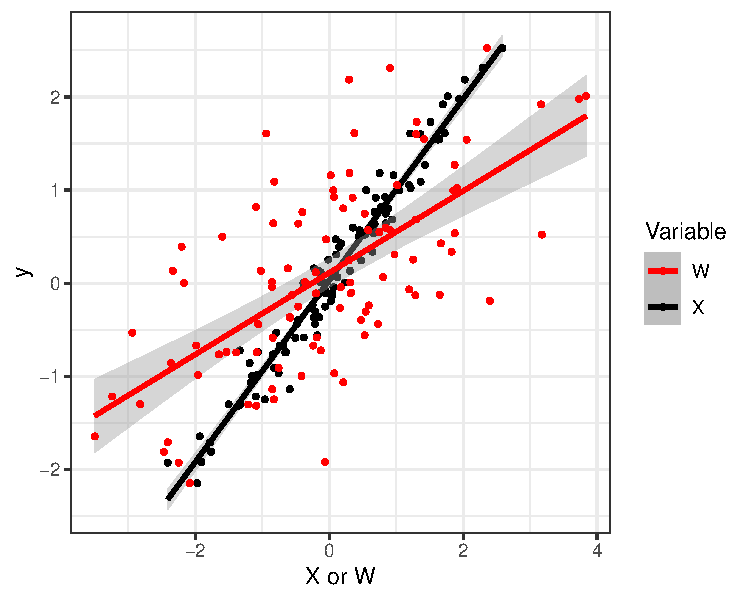
\includegraphics{12Final_files/figure-beamer/unnamed-chunk-2-1.pdf}

\end{frame}

\begin{frame}

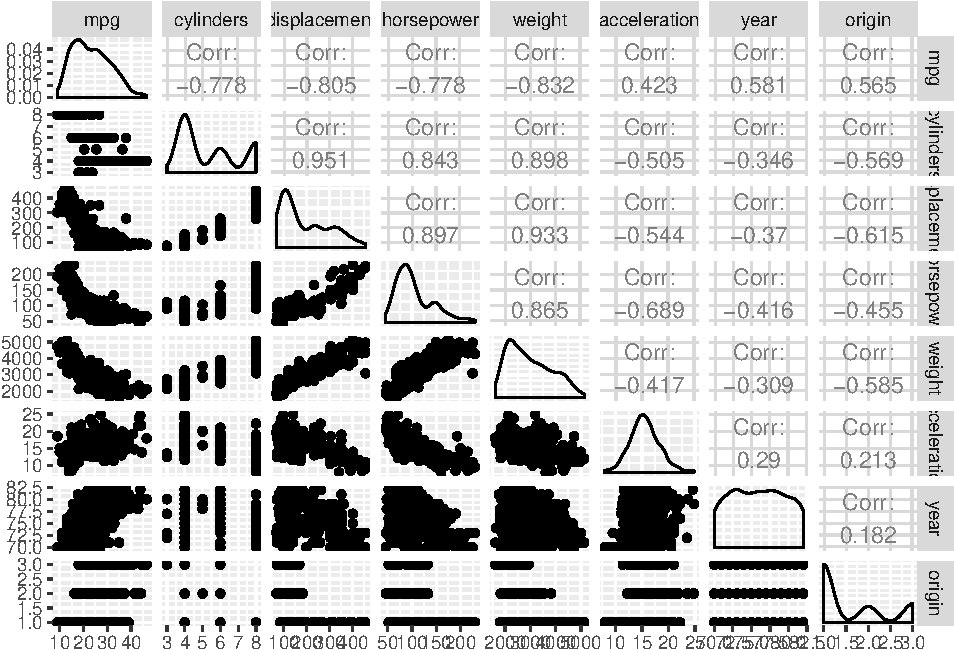
\includegraphics{12Final_files/figure-beamer/unnamed-chunk-3-1.pdf}

\end{frame}

\begin{frame}

Logistic regression gives a probability, given a certain value of the
covariats \(P(Y=1 \, | \, \boldsymbol{x})\).

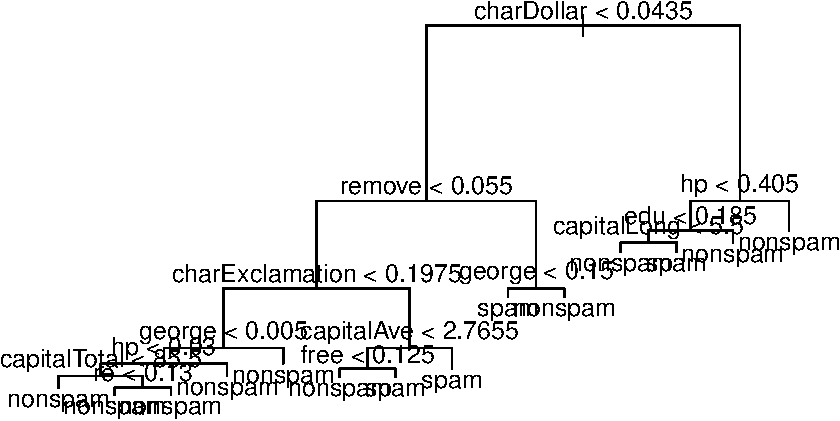
\includegraphics[width=0.9\linewidth]{12Final_files/figure-beamer/unnamed-chunk-4-1}

\end{frame}

\begin{frame}

\begin{block}{5. Resampling methods}

\(~\)

\textbf{Cros-validation}

\begin{itemize}
\tightlist
\item
  Data rich situation: Training-validation and test set.
\item
  Validation set approach
\item
  Cross-validation for regression and for classification.
\item
  LOOCV, 5 and 10 fold CV
\item
  good and bad issues with validation set, LOOCV, 10-fold CV
\item
  bias and variance for \(k\)-fold cross-validation.
\item
  Selection bias -- the right and wrong way to do cross-validation
\end{itemize}

\(~\)

\textbf{The Bootstrap}

\begin{itemize}
\tightlist
\item
  Idea: Re-use the same data to estimate a statistic of interest by
  \emph{sampling with replacement}.
\end{itemize}

\end{block}

\end{frame}

\begin{frame}

\begin{block}{6. Linear model selection and regularization:}

\(~\)

Subset-selection. Discriminate:

\begin{itemize}
\tightlist
\item
  \emph{\textcolor{red}{Model selection}}: estimate performance of
  different models to choose the best one.
\item
  \emph{\textcolor{red}{Model assessment}}: having chosen a final model,
  estimate its performance on new data.
\end{itemize}

\(~\)

How?

\vspace{2mm}

\begin{itemize}
\tightlist
\item
  Model selection by

  \begin{itemize}
  \tightlist
  \item
    Subset selection (best subset selection or stepwise model selection)
  \item
    Penalizing the training error: AIC, BIC, \(C_p\), Adjusted \(R^2\).
  \item
    Cross-validation.
  \end{itemize}
\end{itemize}

\vspace{2mm}

\begin{itemize}
\tightlist
\item
  Model assessment by

  \begin{itemize}
  \tightlist
  \item
    Cross-validation.
  \end{itemize}
\end{itemize}

\end{block}

\end{frame}

\begin{frame}

\begin{itemize}
\item
  Shrinkage methods

  \begin{itemize}
  \tightlist
  \item
    ridge regression: quadratic L2 penalty added to RSS
  \item
    lasso regression: absolute L1 penalty added to RSS
  \item
    no penalty on intercept, not scale invariant: center and scale
    covariates
  \end{itemize}

  \(~\)
\item
  Dimension reduction methods:

  \begin{itemize}
  \tightlist
  \item
    principal component analysis: eigenvectors, proportion of variance
    explained, scree plot
  \item
    principal component regression
  \item
    partial least squares
  \end{itemize}

  \(~\)
\item
  High dimensionality issues: multicollinearity, interpretation.
\end{itemize}

\end{frame}

\begin{frame}

\includegraphics{../../ISLR/Figures/Chapter6/6.7.png}

\end{frame}

\begin{frame}

\includegraphics{../../ISLR/Figures/Chapter6/6.4.png}

\end{frame}

\begin{frame}

\includegraphics{../../ISLR/Figures/Chapter6/6.6.png}

\end{frame}

\begin{frame}

\begin{block}{7. Moving beyond linearity}

\(~\)

\begin{itemize}
\item
  Modifications to the multiple linear regression model - when a linear
  model is not the best choice. First look at one covariate, combine in
  ``additive model''.
\item
  Basis functions: fixed functions of the covariates (no parameters to
  estimate).
\item
  Polynomial regression: multiple linear regression with polynomials as
  basis functions.
\item
  Step functions - piece-wise constants. Like our dummy variable coding
  of factors.
\item
  Regression splines: regional polynomials joined smoothly - neat use of
  basis functions. Cubic splines very popular.
\end{itemize}

\end{block}

\end{frame}

\begin{frame}[fragile]

\begin{itemize}
\item
  Smoothing splines: smooth functions - minimizing the RSS with an
  additional penalty on the second derivative of the curve. Results in a
  natural cubic spline with knots in the unique values of the covariate.
\item
  Local regressions: smoothed \(K\)-nearest neighbour with local
  regression and weighting. In applied areas \texttt{loess} is very
  popular.
\item
  (Generalized) additive models (GAMs): combine the above. Sum of
  (possibly) non-linear instead of linear functions.
\end{itemize}

\end{frame}

\begin{frame}

\includegraphics{../../ISLR/Figures/Chapter7/7.3.png}

\end{frame}

\begin{frame}

\begin{block}{8. Tree-based methods}

\(~\)

\begin{itemize}
\item
  Method applicable both to regression and classification (\(K\)
  classes) and will give non-linear covariate effects and include
  interactions between covariates.
\item
  A tree can also be seen as a division of the covariate space into
  non-overlapping regions.
\item
  Binary splits using only at the current best split: \emph{greedy
  strategy}.
\item
  Minimization criterion: residual sums of squares (RSS), Gini index or
  cross-entropy.
\item
  Stopping criterion: When to stop: decided stopping criterion - like
  minimal decrease in RSS or less than 10 observations in terminal node.
\item
  Prediction:

  \begin{itemize}
  \tightlist
  \item
    Regression: Mean in box \(R_j\)
  \item
    Classification: Majority vote or cut-off on probabiity.
  \end{itemize}
\end{itemize}

\end{block}

\end{frame}

\begin{frame}

\begin{itemize}
\tightlist
\item
  \emph{Pruning}: Grow full tree, and then prune back using pruning
  strategy: cost complexity pruning.
\end{itemize}

To improve prediction (but worse interpretation):

\begin{itemize}
\item
  \emph{Bagging} (bootstrap aggregation): draw \(B\) bootstrap samples
  and fit one full tree to each, used the average over all trees for
  prediction.
\item
  \emph{Random forest}: as bagging but only \(m\) (randomly) chosen
  covariates (out of the \(p\)) are available for selection at each
  possible split. Rule of thumb for \(m\) is \(\sqrt{p}\) for
  classificaton and \(p/3\) for regression.
\item
  Out-of-bag estimation can be used for model selection - no need for
  cross-validation.
\item
  Variable importance plots: give the total amount of decrease in RSS or
  Gini index over splits of a predictor - averaged over all trees.
\item
  \emph{Boosting}: fit one tree with \(d\) splits, make residuals and
  fit a new tree, adjust residuals partly with new tree - repeat.
\end{itemize}

\end{frame}

\begin{frame}

\begin{block}{9. Support vector machines}

\(~\)

\begin{itemize}
\tightlist
\item
  SVM can be used both classification and regression, but we have only
  studied two-class classification.
\end{itemize}

\vspace{2mm}

\begin{itemize}
\tightlist
\item
  Aim: find high dimensional hyperplane that separates two classes
  \(f({\bf x})=\beta_0+{\bf x}^T \boldsymbol\beta=0\). If
  \(y_if({\bf x}_i)>0\) observation \({\bf x}_i\) is correctly
  classified.
\end{itemize}

\vspace{2mm}

\begin{itemize}
\tightlist
\item
  Central: maximizing the distance (on both sides) from the class
  boundary to the closes observations (the margin \(M\)). This was
  relaxed with slack variables (support vector classifiers), and to
  allow nonlinear functions of \({\bf x}\) by extending an inner product
  to kernels (support vector machine).
\end{itemize}

\vspace{2mm}

\begin{itemize}
\tightlist
\item
  Support vectors: observations that lie on the margin or on the wrong
  side of the margin.
\end{itemize}

\end{block}

\end{frame}

\begin{frame}

\begin{itemize}
\item
  Kernels: generalization of an inner product to allow for non-linear
  boundaries and to speed up calculations due to inner products only
  involve support vectors. Most popular kernel is radial
  \[K(x_i,x_i')=\exp(-\gamma\sum_{j=1}^p (x_{ij}-x_{i'j})^2) \ . \]
\item
  Tuning parameters: cost and parameters in kernels - chosen by CV.
\end{itemize}

\vspace{2mm}

\begin{itemize}
\tightlist
\item
  Unfortunately not able to present details since then a course in
  optimization is needed.
\end{itemize}

\vspace{2mm}

\begin{itemize}
\tightlist
\item
  Nice connection to non-linar and ridged version of logistic regression
  - comparing hinge loss to logistic loss - but then without the
  computational advanges of the kernel method.
\end{itemize}

\end{frame}

\begin{frame}

\begin{block}{10. Unsupervised learning}

\(~\)

\begin{itemize}
\tightlist
\item
  Principal component analysis:

  \begin{itemize}
  \tightlist
  \item
    Mathematical details (eigenvectors corresponding to covariance or
    correlation matrix) also in TMA4267.
  \item
    Understanding loadings, scores and the biplot, choosing the number
    of principal components from proportion of variance explained or
    scree-type plots (elbow).
  \end{itemize}
\end{itemize}

\vspace{2mm}

\begin{itemize}
\tightlist
\item
  Clustering:

  \begin{itemize}
  \tightlist
  \item
    \(k\)-means: number of clusters given, iterative algorithm to
    classify to nearest centroid and recalculate centroid
  \item
    hierarchical clustering: choice of distance measure, choice of
    linkage method (single, average, complete),
  \end{itemize}
\end{itemize}

\end{block}

\end{frame}

\begin{frame}

\centering

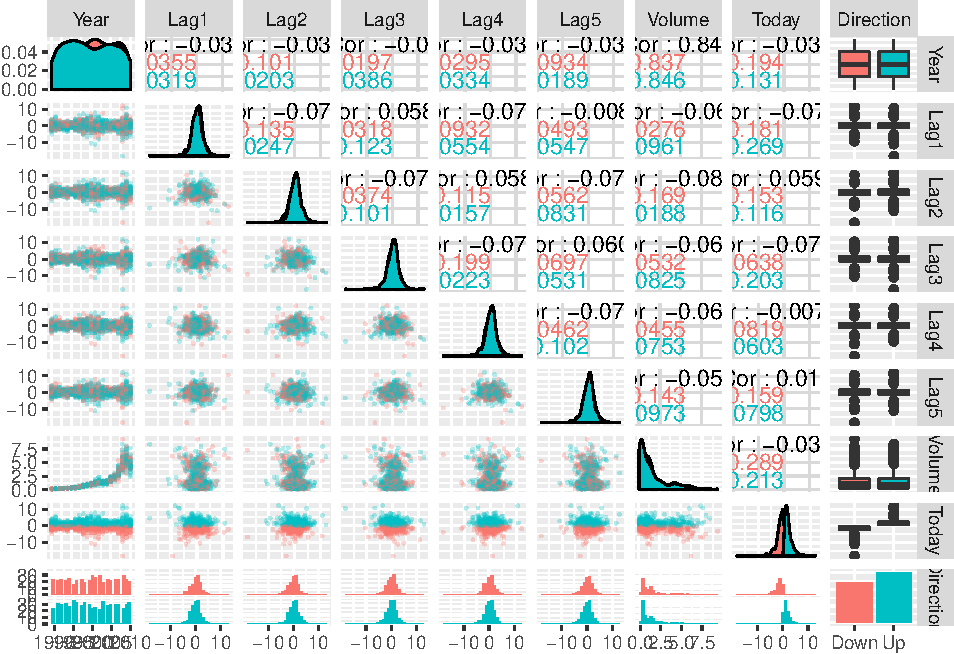
\includegraphics[width=0.7\linewidth]{12Final_files/figure-beamer/unnamed-chunk-5-1}

\end{frame}

\begin{frame}

PCA for quality control

\centering

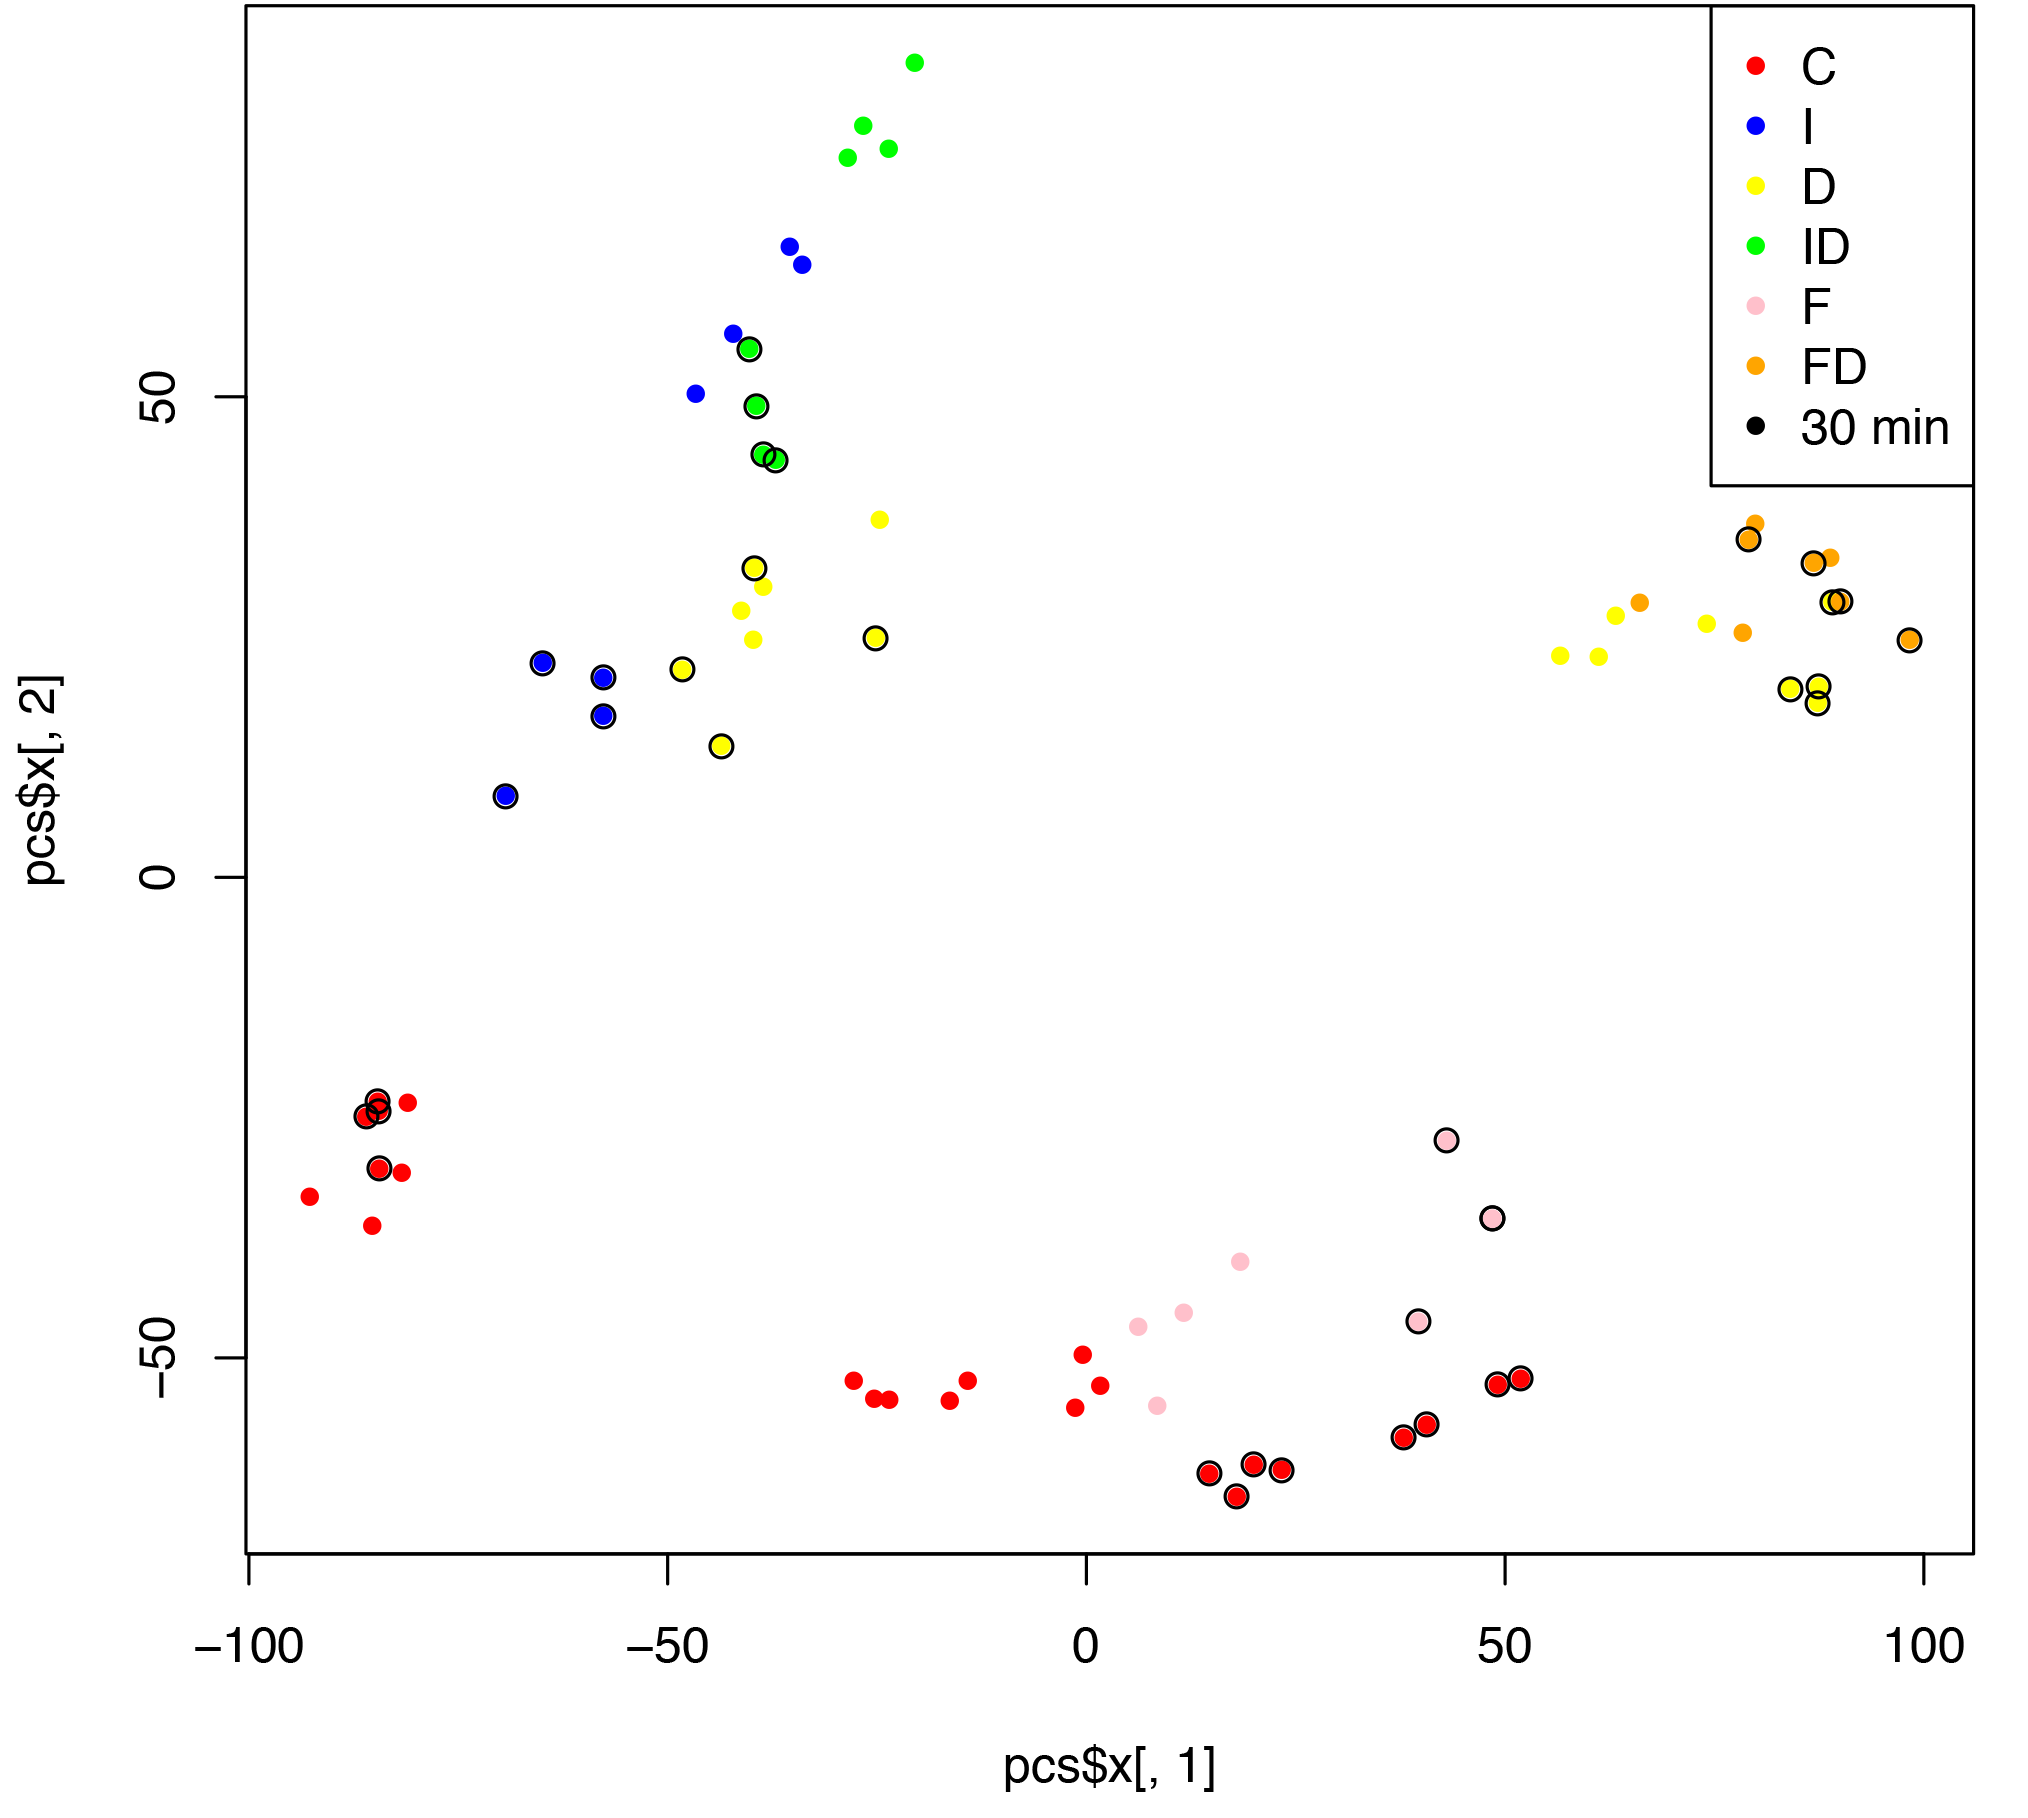
\includegraphics[width=0.8\textwidth,height=\textheight]{PCAforQC.png}

\end{frame}

\begin{frame}

Hierarchical clustering for visualization

\centering

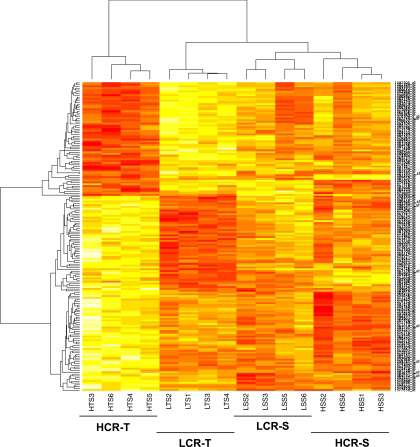
\includegraphics[width=0.7\textwidth,height=\textheight]{../1Intro/heatmap.png}

\end{frame}

\begin{frame}[fragile]

\begin{block}{11. Neural networks}

\begin{block}{Topics in Module 11:}

\begin{itemize}
\tightlist
\item
  Feedforward network architecture: mathematical formula - layers of
  multivariate transformed (\texttt{relu}, \texttt{linear},
  \texttt{sigmoid}) inner products - sequentially connected.
\item
  What is the number of parameters that need to be estimated? Intercept
  term (for each layer) is possible and is referred to as ``bias term''.
\item
  Loss function to minimize (on output layer): regression (mean
  squared), classification binary (binary crossentropy), classification
  multiple classes (categorical crossentropy) --- and remember to
  connect to the correct choice of output activiation function: mean
  squared loss goes with linear activation, binary crossentropy with
  sigmoid, categorical crossentropy with softmax.
\item
  How to minimize the loss function: gradient based (chain rule)
  back-propagation - many variants.
\end{itemize}

\end{block}

\end{block}

\end{frame}

\begin{frame}[fragile]

\begin{itemize}
\tightlist
\item
  Technicalities: \texttt{nnet} in R
\item
  Optional (not on reading list): \texttt{keras} in R. Use of tensors.
  Piping sequential layers, piping to estimation and then to evaluation
  (metrics).
\end{itemize}

\end{frame}

\begin{frame}{After TMA4268 - what is next?}
\protect\hypertarget{after-tma4268---what-is-next}{}

What are the statistical challenges we have not covered?

Do you want to learn more about the methods we have looked at in this
course? And also methods that are more tailored towards specific types
of data? Then we have many statistics courses that you may choose from.

An overview of statistics courses and also information on the statistics
staff (for bachelor and master supervision)
\url{https://folk.ntnu.no/mettela/Talks/3klinfo20190325.html}

\end{frame}

\begin{frame}

On behalf of the teaching staff - Michail, Andreas, Thiago and Mette-

\textbf{thank you for attending this course - hope to see you for the
exam supervision - and good luck on May 23!}

\end{frame}

\begin{frame}{References}
\protect\hypertarget{references}{}

\hypertarget{refs}{}
\leavevmode\hypertarget{ref-ISL}{}%
James, Gareth, Daniela Witten, Trevor Hastie, and Robert Tibshirani.
2013. \emph{An Introduction to Statistical Learning}. Vol. 112.
Springer.

\leavevmode\hypertarget{ref-james.etal}{}%
James, G., D. Witten, T. Hastie, and R. Tibshirani. 2013. \emph{An
Introduction to Statistical Learning with Applications in R}. New York:
Springer.

\end{frame}

\end{document}
